\section{A tools provider's perspective: Iterative.ly}
\label{section-tool-providers-perspective}
The use of mobile analytics extends beyond the development role in a team or organisation. Software tools should also serve the project rather than being the master of it. ~\citep{budgen1993_case_tools_masters_or_servants} raises a similar issue of whether CASE tools are masters or servants. There is a significant risk that development teams lose control of the data, and/or are constrained by the policies, implementation, and so on of a particular tool provider. Companies including Iteratively, Avo, and Segment aim to provide aspects of: freedom of choice and the ability to choose, cross team alignment and visibility of the use of embedded (in-app) analytics, and compliance. Here, Iteratively is included as a mini case-study of what one of these companies is doing to help development teams in their use of embedded (in-app) mobile analytics.

%Cross team tracking and alignment on the use of embedded (in-app) mobile analytics 

%Introduce the company: location, age, type of business, etc. Information freely given with permission to use it generally, including for research purposes.
Iteratively was founded on \nth{20} February 2019 and based in Seattle, Washington State, USA by two experienced co-founders. They contacted me in May 2020 as they were interested in my perspective and research into mobile analytics. %Sources include: https://iterative.ly/about/ https://www.crunchbase.com/organization/iteratively
%
Subsequently, they kindly agreed to contribute to this research as a small case study of a startup aiming to develop products to help development teams improve their use of mobile analytics. They provided all information is freely given with permission to use it generally, including for research purposes.

This research case study include these research methods: semi-structured interviews, a walk-through of the tools and service, collaborative verbal discussions and various written materials.

Their service is self-described as ``GitHub for your analytics", providing a versioned schema registry for analytics events~\footnote{Source: a non-public document used with permission.}.
%
Their value proposition: a versioned schema for web and mobile analytics. Tools that generate the client-side SDK that developers then include in their apps. They use lint tools to verify that events have been instrumented correctly. At runtime their SDK validates event payloads match the schema to help enforce data quality. They provide tools that help detect some forms of PII with the aim of helping improve legal compliance.  

Relevance to the research in the thesis: tools to help design and validate the analytics content. A whitebox insight into an analytics provider who also develop and provide tools to help organisations improve their use of mobile and web analytics. 


\subsection{Related work}
- Mention similar work avo.app
- segment.io - indicates the growth and relevance of mobile analytics as a market, of addressing data ownership and freedom of choice of analytics implementations. 

\subsection{Their market research}
MUST-DO expand this section, mainly to cover key points in their early market research and the relevance to the research in this thesis.

What leading edge businesses value in their analytics tools? (10 dots voting examples, see Figure~\ref{tab:10dots_voting_iteratively}), their early market research (see the first notion.io document.)


Dot voting is a simple voting exercise where each participant has a finite number of dots they can vote with to prioritise a set of choices~\citep{18f_dot_voting}. Dot voting is used in many software development teams who use Agile software development practices, and offers easy and lightweight voting of ideas~\citep{nngroup_dot_voting}. There are criticisms of the technique, for instance where poorly designed options split votes, where people vote tactically, or where people appropriate and use dots from others~\citep{dotmocracy}. The approach used by iteratively mitigates against these concerns through the design and implementation of the voting. 

Iteratively's method uses a video call with screen sharing. Each participant has already agreed to take part in the research exercise which includes the ten dots voting as part of a semi-structured interview. They are presented with the prepared template `Spend 10 coins', as illustrated in Figure~\ref{fig:iteratively-spend-10-dots}. The interviewer explains each item in order until each of them have been explained. Some interviewees allocate the coins (dots) early others wait until the end of the explanation.


\begin{figure}[htbp!]
    \centering
    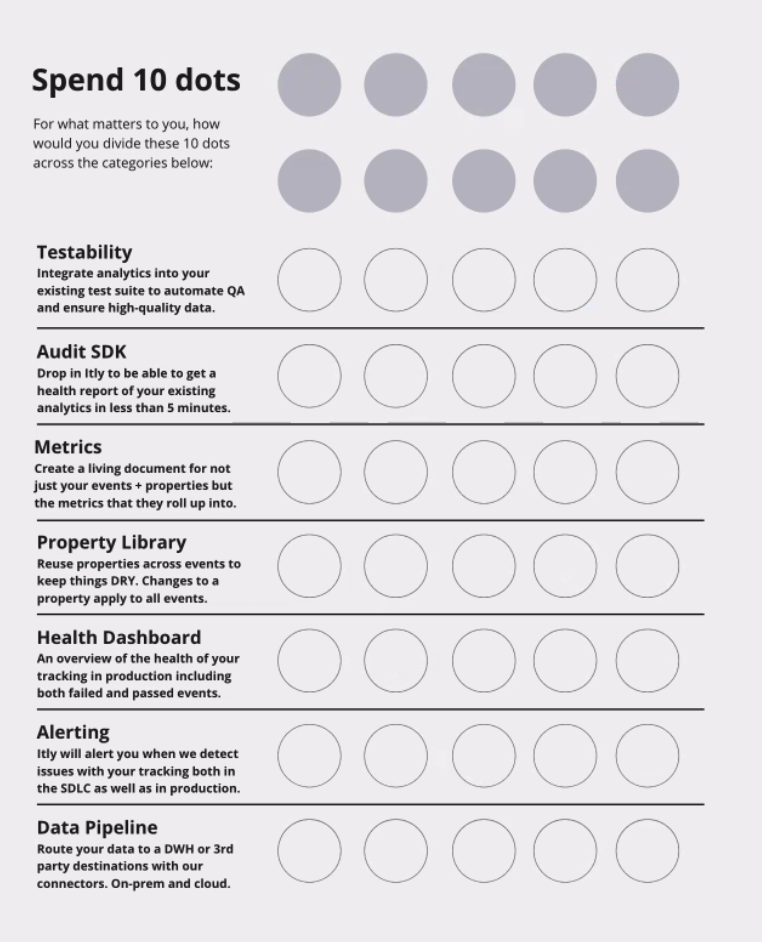
\includegraphics[width=10cm]{images/iteratively/spend-10-dots.png}
    \caption{Interatively spend 10 dots}
    \label{fig:iteratively-spend-10-dots}
\end{figure}

According to Iteratively the votes are helpful, and the discussions around the topics more so.  Figure~\ref{fig:iteratively-dot-voting-example} is an example where the votes have been cast. 

\begin{figure}[htbp!]
    \centering
    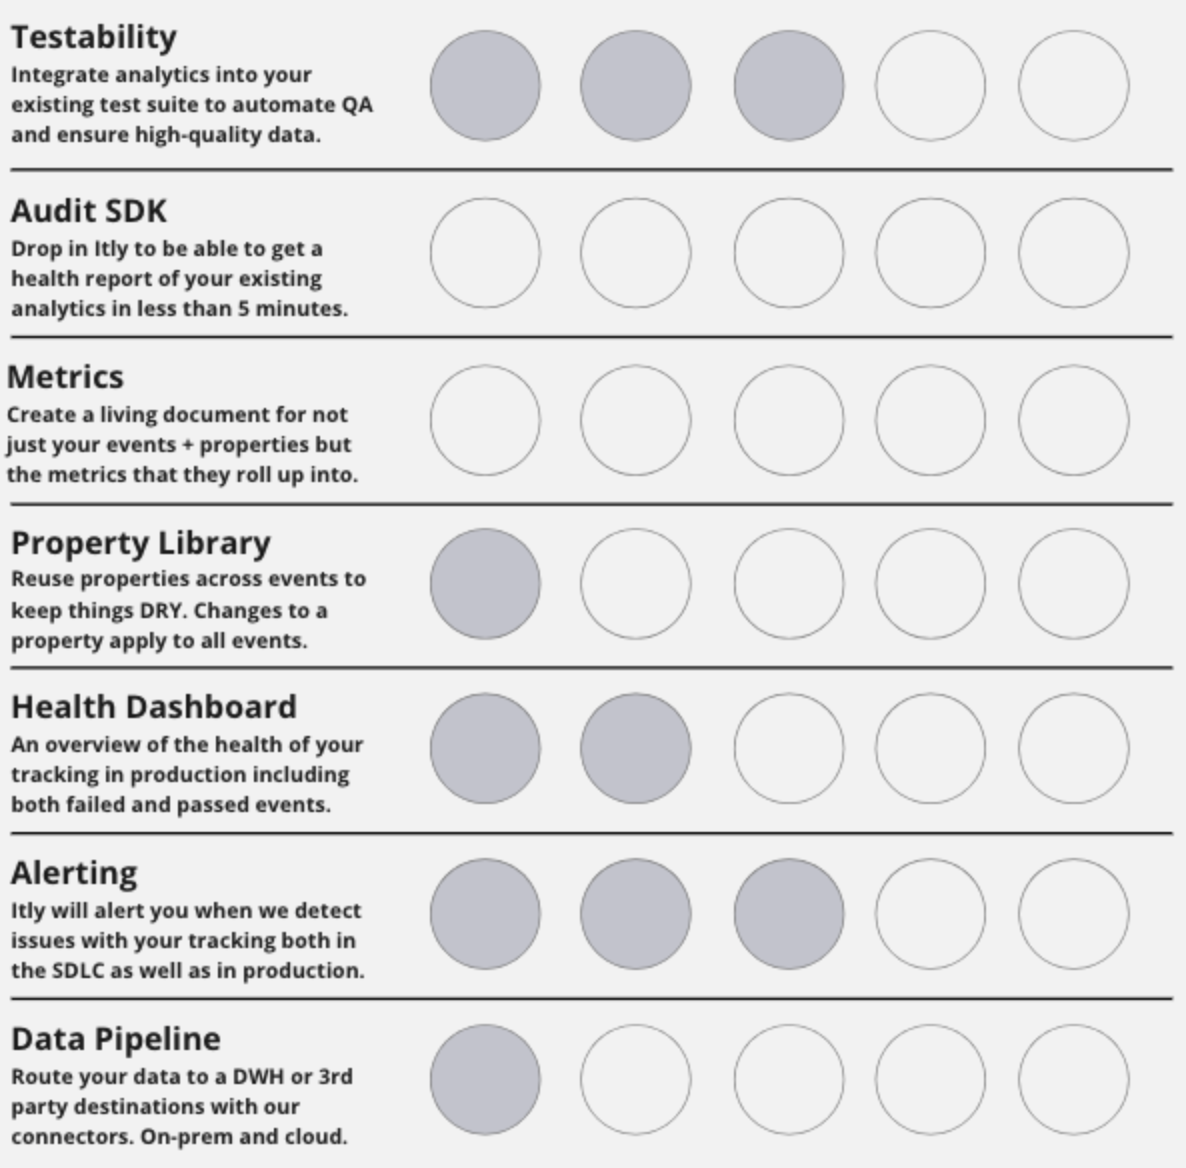
\includegraphics[width=10cm]{images/iteratively/dot-voting-example.png}
    \caption{Iteratively dot voting example}
    \label{fig:iteratively-dot-voting-example}
\end{figure}


Seven candidate topics were used, here are the exact wordings of each topic description:
\begin{enumerate}
    \item \textbf{Testability}: Integrate analytics into your existing test suite to automate QA and ensure high-quality data.
    \item \textbf{Audit SDK}: Drop in itly\footnote{itly: Iteratively.} to be able to get a health report of your existing analytics in less than 5 minutes.
    \item \textbf{Metrics}: Create a living document for not just your events + properties but the metrics they roll up into.
    \item \textbf{Property Library}: Reuse properties across events to keep things DRY. Changes to a property apply to all events.
    \item \textbf{Health Dashboard}: An overview of the health of your tracking in production including both failed and passed events.
    \item \textbf{Alerting}: Itly will alert you when we detect issues with your tracking both in the SDLC\footnote{SDLC: Software Development Life Cycle.} as well as in production.
    \item \textbf{Data Pipeline}: Route your data to a DWH\footnote{DWH: Data Warehouse.} or 3rd party destinations with our connectors. On-prem~\footnote{On-prem: On premise.} and cloud.
\end{enumerate}
These topics were chosen to help Iteratively with planning their product roadmap. They also provide a useful context and perspective for the research into using mobile analytics from product and data engineering perspectives. With one exception, all the participants actively use analytics in their software and have expressed an interest in improving their approach into incorporating and using analytics in their apps.

\begin{table}[htbp!]
 
    \centering
    \small
    \setlength{\tabcolsep}{4pt} %% default is 6pt
    %% With thanks to http://tex.my/how-to-deal-with-wide-tables/ for the \tabcolsep tip
    \begin{tabular}{lr|rrrrrrrrrrrrrr}
    % SHOULD-DO Added column span over the participants, reduce the heavy lines on the table.
                     &Sum &A  &B  &C  &D  &E  &F  &G  &H  &I  &J &K &L &M &N\\
    \hline     
    Testability         &30 &3  &3  &3  &1  &   &3  &3  &1  &5  &3 &  &3 &1 &1\\
    Audit SDK           &25 &   &2  &   &   &2  &2  &3  &1  &2  &1 &3 &3 &5 &1\\
    Metrics             &6  &   &   &   &   &   &1  &   &   &   &  &  &1 &3 &1\\
    Property library    &21 &1  &3  &3  &2  &3  &2  &1  &   &   &1 &1 &1 &  &3\\
    Health Dashboard    &17 &2  &   &2  &   &3  &   &2  &2  &   &2 &2 &  &1 &1\\
    Alerting            &18 &3  &2  &   &2  &   &2  &   &4  &   &3 &  &1 &  &1\\
    Data Pipeline       &18 &1  &   &2  &   &2  &   &1  &2  &3  &  &4 &1 &  &2\\
         
    \end{tabular}
    \caption{10 dots voting Iteratively market research}
    \label{tab:10dots_voting_iteratively}

\end{table}
% My spreadsheet https://docs.google.com/spreadsheets/d/1Acti8klc6JvLu_NAR7t7cC8XdMHx-FIkfSHcqt_srwc/edit#gid=0 
% Source from iterative.ly's miro board https://miro.com/app/board/o9J_kujB-Y4=/ 

The first ten sets of dot votes rank the choices as follows: Testability (25), Property Library (16), Alerting (16), Audit SDK (13), Health Dashboard (13), Data Pipeline (11), and lastly Metrics (1). The next three sets of dot votes cement testability as the \#1 ranking, they also bump up auditing the use of the SDK to second place in the rankings, and even metrics gets a boost to 5 votes in total. 

With 14 sets of votes, the ranking is still volatile and the scores unlikely to be sufficiently robust to depend on. Nonetheless several indications are starting to emerge. 
These votes indicate testability is the most desired property for designing and implementing analytics where the analytics can help shape and drive automated testing of software based on production usage characteristics. Auditing of the SDK is in a strong second place, to provide an immediate health check of the existing analytics. Participants who use Iteratively's services score property library highly as they have experienced the value in this capability. Alerting when issues are detected with the tracking in the SDLC and production ties in joint fourth place with the data pipeline. Data pipeline is more important than it may appear, as some of the respondents professed they preferred alternatives to using Iteratively to provide the data pipeline. The interviews indicated that data pipelines are more important than the score indicates.

The seven topics were chosen quickly and not necessarily intended to be comprehensive. One omission we discussed is the area that encompasses: privacy, Personally Identifiable Information (PII), and compliance, nonetheless these are believed to be important to Iteratively's current and potential customers and an area they are actively working on.

\subsection{Evaluation of their service}
SHOULD-DO apply their tooling for an Android app for an existing app and discuss the effects of using their tooling and service. % Possibly do this with Joe Reeve to include his perspective as he transitions from outsider to insider at the company?

\subsection{Indications of where mobile analytics is heading}
Iteratively and several companies with similar value propositions indicate several potential trends in the use of mobile analytics. These trends include: mobile analytics is now subject to quality criteria, where organisations seek mechanisms to help them integrate mobile analytics as a first-class citizen in app development, potentially at least as valuable as some features in their apps. Also there is a need and a desire to use and manage mobile analytics effectively, including ownership and management of the data that is collected by the many and various mobile analytics tools. 

% Call notes with Patrick Fri 30th April 2021 30 mins, 16:00 BST
% He's keen to read my thesis and provide feedback.
% He's fine with him and with Joe providing details and me picking Joe's brains about Iteratively and the products. 
% He's also keen to give back in terms of the help and advice I've provided
